\documentclass{report}

%% Required packages
\usepackage[utf8]{inputenc}
\usepackage[T1]{fontenc}
\usepackage{lmodern}
\usepackage{amsmath,amssymb,amsthm,dsfont}

%% Page layout
\usepackage[margin=1in]{geometry}
\usepackage{setspace}

%% Graphics and figures
\usepackage{graphicx}
\usepackage{caption}
\usepackage{subcaption}
\usepackage{tikz}
\usetikzlibrary{patterns}
\usepackage{pdfpages}

%% Tables and formatting
\usepackage{booktabs}
\usepackage{makecell}
\usepackage{tabularx}
\usepackage{array}
\usepackage{lscape}
\usepackage[capposition=top]{floatrow}

%% Colors and fonts
\usepackage{xcolor}

%% Table of contents and formatting
\usepackage[nottoc,notlof,notlot]{tocbibind}
\usepackage{titlesec}
\usepackage[titles]{tocloft}
\setlength{\cftbeforechapskip}{4pt}
\renewcommand\cftfigafterpnum{\vskip1.5pt\par}
\renewcommand\cfttabafterpnum{\vskip1.5pt\par}
\cftsetindents{figure}{0em}{3.5em}
\cftsetindents{table}{0em}{3.5em}

%% Formatting for chapters, sections, and subsections

\titleformat{\chapter}[display]{\normalfont\Large\bfseries\centering}{\chaptertitlename\ \thechapter}{10pt}{\Large} 
\titlespacing*{\chapter}{0pt}{0pt}{35pt}
\titlespacing*{\section}{0pt}{2.5ex}{2.5ex}
\titlespacing*{\subsection}{0pt}{2.5ex}{2.5ex}
\titlespacing*{\subsubsection}{0pt}{2.5ex}{1.5ex}

\setcounter{secnumdepth}{3} % how many sectioning levels to assign numbers to


%% URL and hyperlinks
\usepackage{hyperref}
\hypersetup{
    colorlinks=true,
    linkcolor=blue,
    filecolor=blue,      
    urlcolor=blue,
    breaklinks = true,
    citecolor = blue
}
\urlstyle{same}

%% Enumeration

\usepackage{enumerate}
\usepackage[inline]{enumitem}

%% Bibliography

\usepackage[backend = biber,
			maxnames = 10,
			maxcitenames = 3,
			maxbibnames = 10,
			minbibnames = 1,
			doi = false,
			eprint = false,
			style = apa
			]{biblatex}
\setlength\bibitemsep{1.25\itemsep}
\addbibresource{biblio.bib}

\setlength{\parskip}{.5em}%

\graphicspath{{chapter_one/}{chapter_one/}{chapter_three/}}

\renewcommand{\contentsname}{TABLE OF CONTENTS}
\renewcommand{\listfigurename}{LIST OF FIGURES}
\renewcommand{\listtablename}{LIST OF TABLES}
\renewcommand{\chaptername}{CHAPTER}

% Common Math-related commands
%% More commands in main.tex for each chapter

\newtheorem{assu}{Assumption}
\newtheorem{prop}{Proposition}
\newtheorem{definition}{Definition}

\DeclareMathOperator{\Var}{\mathbb{Var}}
\DeclareMathOperator{\Corr}{\mathbb{Corr}}
\DeclareMathOperator{\Cov}{\mathbb{Cov}}
\DeclareMathOperator{\E}{\mathbb{E}}

\newcommand{\pre}{\text{Pre}}
\newcommand{\post}{\text{Post}}

%% University details
\newcommand{\university}{University Name}
\newcommand{\department}{Department of Something}

%% BEGIN DOCUMENT %%%%%%%%%%%%%%%%%%%%%%%%%%%%%%%%%%%%%%%%%%%%%%%%%%%%%%%%%%%%%%

\begin{document}

\begin{titlepage}
    \begin{center}
        \vspace*{0.5cm}
        \linespread{1.3}
        
        \LARGE
        \textbf{Triumph and Transformation: Messi's Journey in Club and International Football}
        
        \vspace{2.5cm}
        
        \normalsize
        By
        
        \vspace{1cm}
        \large Author Name \\
        \vspace{0.25cm}
        \normalsize
        B.A., Universidad de Rosario, 2017 \\
        M.A., \university, 2024
            
        \vspace{3cm}
        \large

        A Dissertation Submitted in                           \\
        Partial Fulfillment of the Requirements for           \\
        the Degree of Doctor of Philosophy in the             \\
        \department\ at \university
            
        \vspace{4.5cm}
        
        City, State or Province \\
        Month YYYY
            
    \end{center}
\end{titlepage}

\newpage
\pagenumbering{gobble}
\begin{minipage}[b]{0.9\textwidth}\centering
\vspace{0.45\textheight}
\textcopyright{} Copyright 2024 \\
by Author Name
\end{minipage}

\newpage
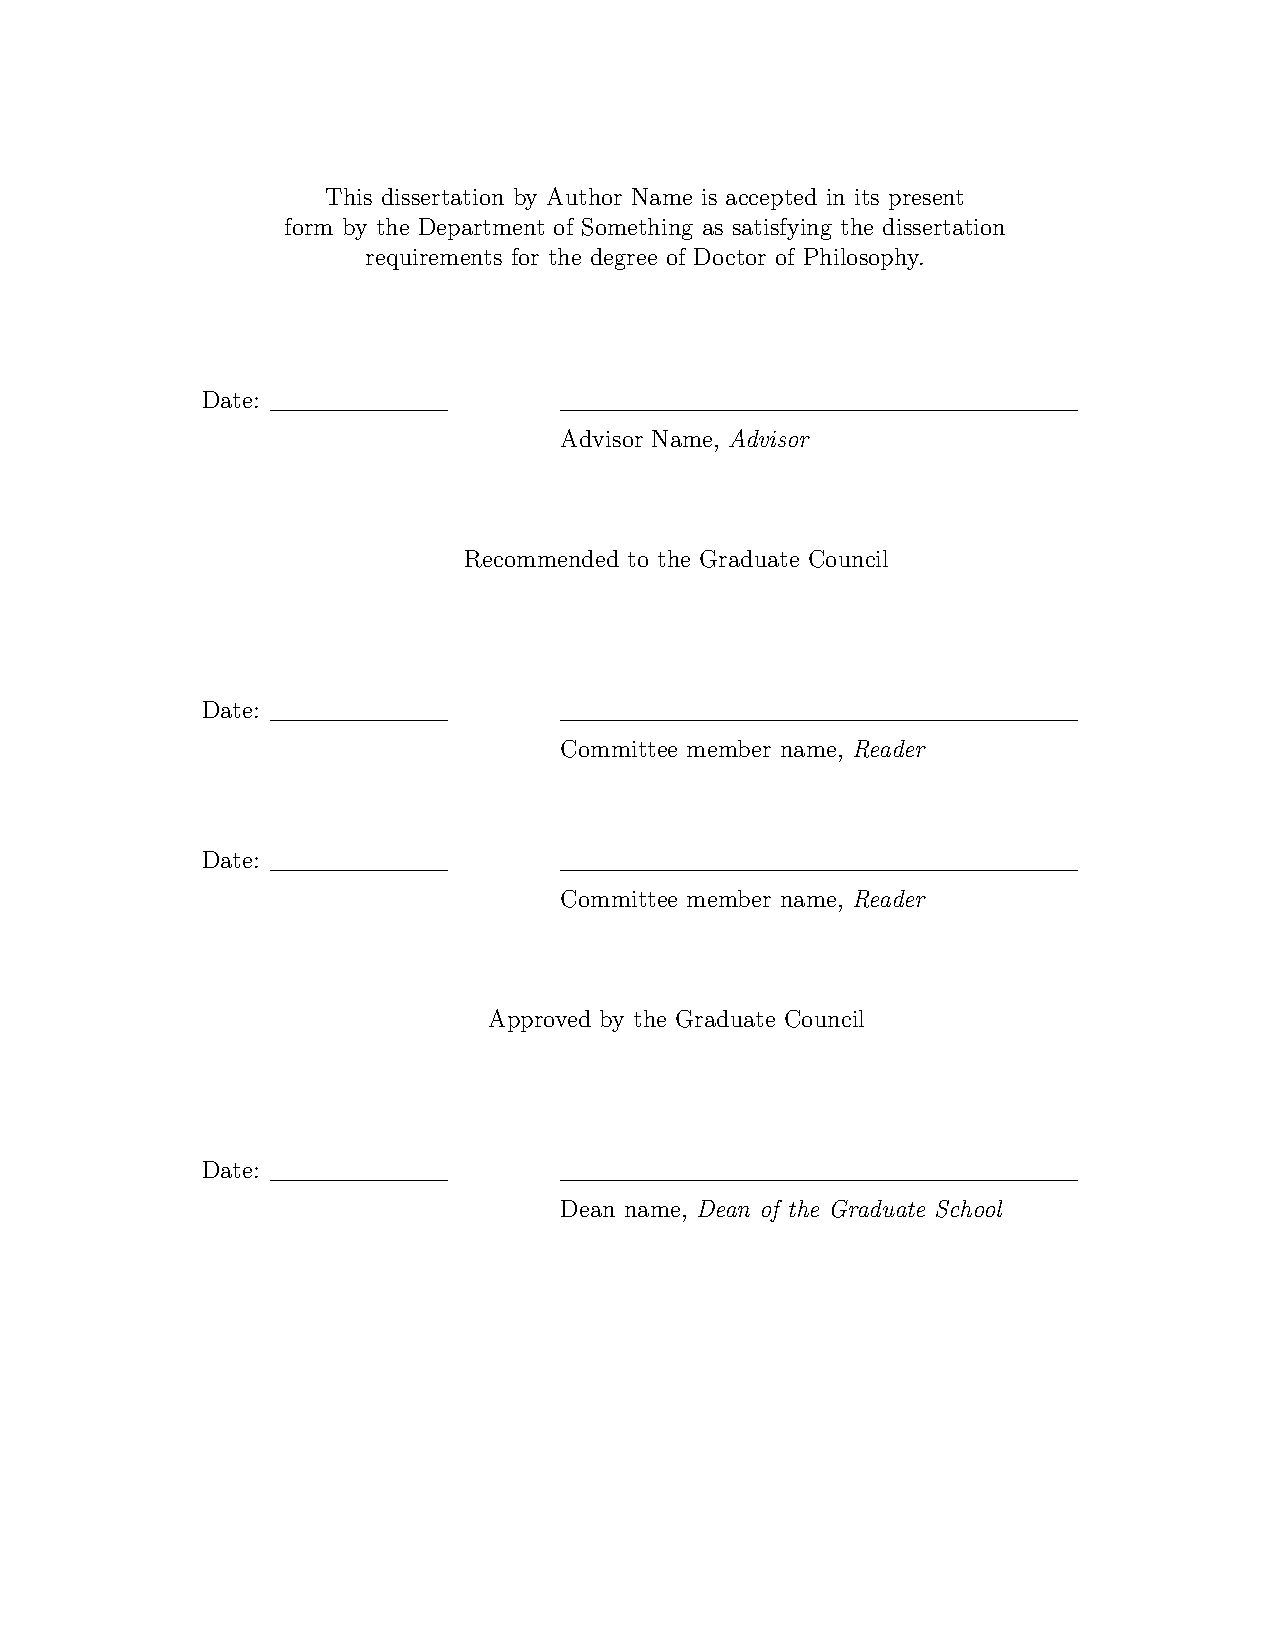
\includepdf{signature_page/page.pdf}

\doublespacing
\pagenumbering{roman}
\pagestyle{plain}
\setcounter{page}{4}

\chapter*{CURRICULUM VITAE}

The author is originally from Rosario, Santa Fe, Argentina.
He completed his undergraduate studies at the \textit{Universidad de Rosario},
where he worked as a Research Assistant.
Before starting his PhD, he worked in WORK EXPERIENCE.
In 2018, he entered the PhD program in \department\ at \university.
He is a football fan.

\chapter*{ACKNOWLEDGEMENTS}

I thank my family and friends for their support.

I thank my colleagues for the discussions and feedback.

I thank my committee for the invaluable guidance.

\chapter*{PREFACE}

The life of Lionel Messi embodies the pinnacle of footballing achievement. 
His otherworldly talent captivated the world, shattering records while leading 
FC Barcelona and the Argentina national team to countless victories.
This dissertation delves into Messi's remarkable journey, providing a 
comprehensive analysis of his extraordinary career.

Beginning with his meteoric rise at Barcelona, this work examines Messi's 
iconic goals, titles, and the transformative impact he had on the sport.
It then explores his triumphs---and heartbreaks---with Argentina, culminating in 
his ultimate conquest: winning the World Cup.
Finally, the dissertation analyzes Messi's continued evolution on the pitch 
at Paris Saint-Germain and the potential future role with Inter Miami.

\setcounter{tocdepth}{1} % Set the depth of the table of contents

\tableofcontents
\listoftables
\listoffigures


%% CHAPTER ONE %%%%%%%%%%%%%%%%%%%%%%%%%%%%%%%%%%%%%%%%%%%%%%%%%%%%%%%%%%%%%%%%%
\clearpage

\pagenumbering{arabic}% Arabic page numbers (and reset to 1)
\setcounter{page}{1}
\doublespacing

\setcounter{section}{0}% Reset section counter

\chapter{The FC Barcelona years}


\section{Introduction}\label{sec:chap1_intro}
 
Lionel Messi's ascension from a gifted youth prospect to a global football icon 
unfolded over a remarkable period at FC Barcelona.
His time with the Catalan giants serves as a testament to both extraordinary 
talent and unwavering dedication, ultimately elevating him to a status few 
athletes ever achieve. 

This chapter examines the formative years of Messi's legendary career.
By analyzing his performances, his unparalleled success in winning titles, and 
the transformative impact he had on FC Barcelona, the groundwork for 
understanding his enduring influence on the sport is established.
His successes are reflected in titles, such as \textcite{messi2011ucl} 
and \textcite{messi2015ucl}, and in astounding individual performances
\parencite[e.g,][]{messi2009clasico}.

This exploration sets the stage for the dissertation's subsequent analysis of 
Messi's continued evolution throughout his career, 
including the challenges and triumphs he faced beyond Barcelona's hallowed grounds. 

This chapter is organized as follows. 
Section \ref{sec:chap1_background} provides background information on Messi's 
early years at FC Barcelona.
Section \ref{sec:chap1_titles} presents an overview of the titles Messi won 
during his time at the club.
Section \ref{sec:chap1_performance} analyzes Messi's performance metrics during 
his tenure at FC Barcelona.

\section{Background}\label{sec:chap1_background}

Lionel Messi joined FC Barcelona's youth academy, La Masia, at the age of 13.
His prodigious talent was evident from an early age, and he quickly rose through
the ranks of the club's youth system.

Messi made his first-team debut for Barcelona in 2004, at the age of 17, under 
the coaching of Frank Rijkaard.
He quickly established himself as a key player for the club, showcasing his
remarkable dribbling ability, vision, and goal-scoring prowess.

In fact, Messi's first goal for Barcelona came on May 1, 2005, in a match 
against Albacete.
In the 88th minute of the game, Messi received a pass from Ronaldinho and 
skillfully put the ball above the goalkeeper to celebrate his first goal.
At just 17 years and 10 months old, Messi became the youngest goal scorer in 
the history of the club.

\section{Titles}\label{sec:chap1_titles}

During his time at FC Barcelona, Lionel Messi won numerous titles, as depicted
in Table \ref{tab:messi_barca_titles}.
These include multiple La Liga titles, UEFA Champions League titles, and Copa del Rey
titles.

\begin{table}[ht!]
    \centering
    \caption{Lionel Messi's Titles with FC Barcelona}
    \begin{tabular}{|c|c|}
    \hline
    \textbf{Competition} & \textbf{Number of Titles} \\ \hline
    La Liga & 10 \\ \hline
    Copa del Rey & 7 \\ \hline
    UEFA Champions League & 4  \\ \hline
    \end{tabular}
    \label{tab:messi_barca_titles} 
\end{table}
    

His position in the field and playing style evolved over the years, as 
different coaches utilized his talents in various ways.
For example, under Pep Guardiola, Messi played as a false nine, dropping deep
to create space for his teammates and exploit opposition defenses.
This constant evolution and adaptation to different roles on the field
demonstrate Messi's versatility and footballing intelligence, and were 
key to his success at Barcelona.

\begin{table}[ht!]
    \centering
    \caption{Goals and Assists by Lionel Messi Each Year in FC Barcelona}
    \begin{tabular}{ccc}
      \hline
      Season & Goals & Assists \\ \hline
      2004-05 & 9 & 1 \\
      2005-06 & 25 & 8 \\
      2006-07 & 36 & 17 \\
      2007-08 & 40 & 16 \\
      2008-09 & 51 & 38 \\
      2009-10 & 53 & 47 \\
      2010-11 & 55 & 53 \\
      2011-12 & 60 & 73 \\
      2012-13 & 50 & 60 \\
      2013-14 & 46 & 41 \\
      2014-15 & 58 & 57 \\
      2015-16 & 49 & 41 \\
      2016-17 & 52 & 54 \\
      2017-18 & 54 & 45 \\
      2018-19 & 50 & 51 \\
      2019-20 & 44 & 31 \\
      2020-21 & 47 & 38 \\
    \hline
    \end{tabular}
    \label{tab:messi_barca_goals_assists}
\end{table}
  

\section{Performance}\label{sec:chap1_performance}

The performance of Lionel Messi during his tenure at FC Barcelona is 
nothing short of extraordinary.
His goal-scoring and playmaking abilities have earned him numerous 
accolades and titles.
Table \ref{tab:messi_barca_goals_assists} showcases Messi's remarkable 
goal and assist statistics, highlighting his immense contribution to the 
team's success.

Messi had a record-breaking calendar year in 2012, scoring 91 goals in all 
competitions.
This peak performance is illustrated in Figure \ref{fig:messi_goals_xg_2012}, 
which shows the ratio of goals to expected goals (xG) for Messi and other players
in the 2012/13 season.
Messi consistently outperformed his xG, demonstrating his exceptional finishing
ability and efficiency in front of goal.

\begin{figure}[ht!]
    \centering
    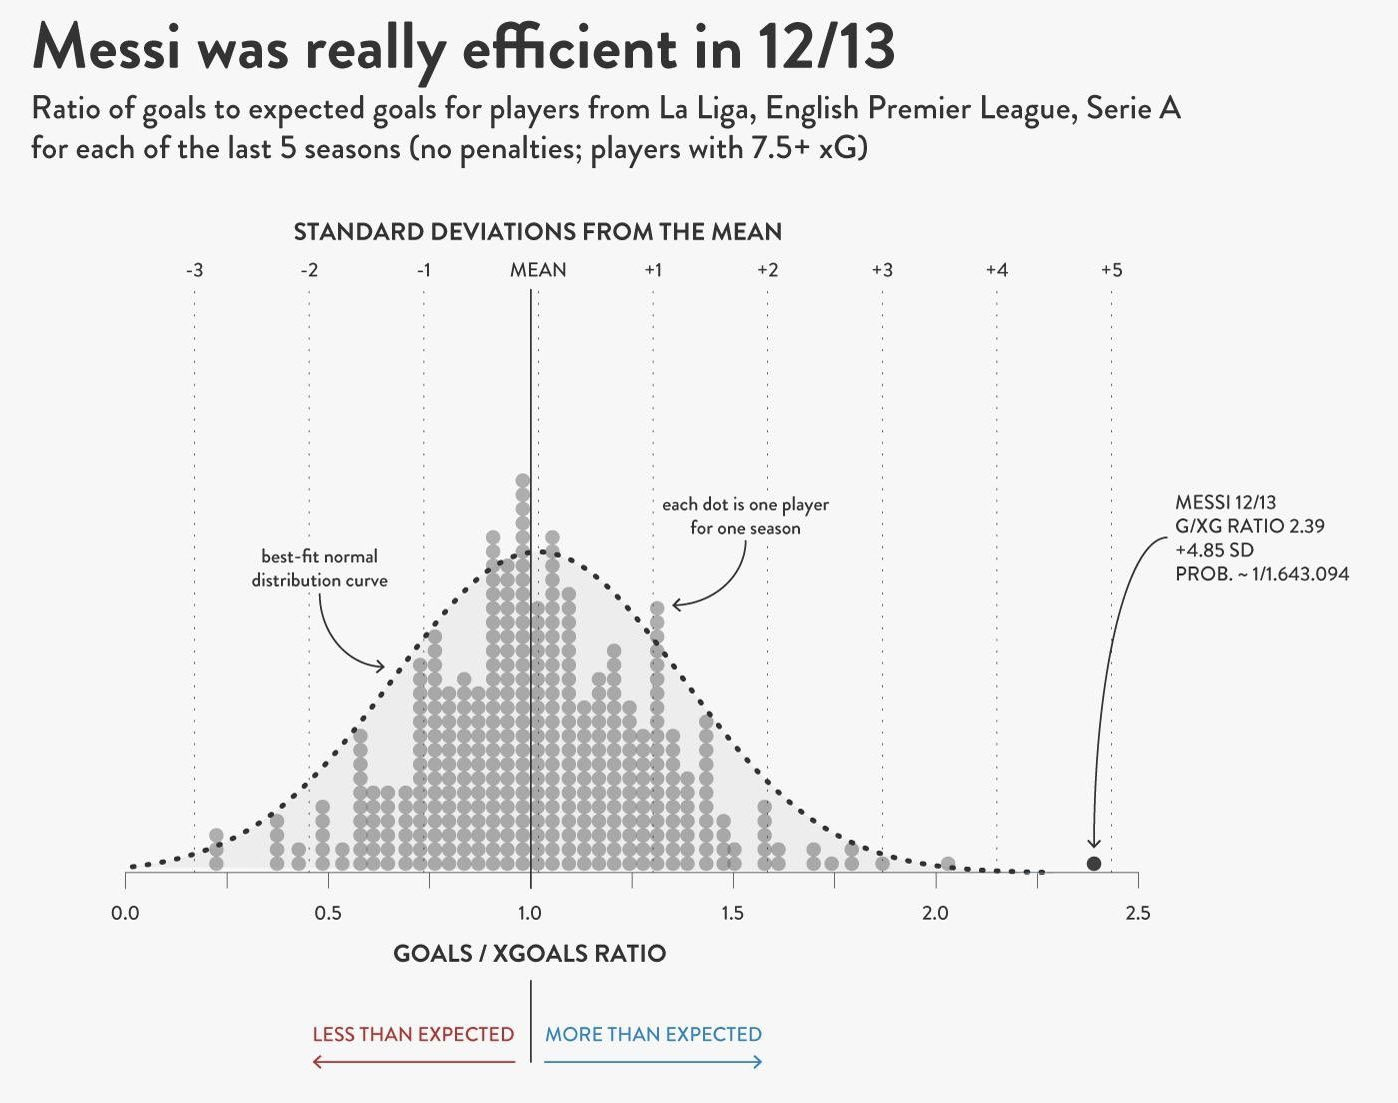
\includegraphics[width=0.7\textwidth]{graphics/messi_2012.jpg}
    \caption{Messi's Exceptional Finishing in 2012/13}
    \label{fig:messi_goals_xg_2012}
    \begin{quote}
        \textit{Notes:} 
        The figure shows the ratio of goals to expected goals (xG) for several 
        players in the 2012/13 season.
        \textit{Source:} Twitter, @xGPhilosophy.
    \end{quote} 
\end{figure}


Messi was coached by some of the best managers in the world during his time at
Barcelona, including Pep Guardiola, Luis Enrique, and Ronald Koeman.
A key aspect of Messi's success was his ability to adapt to different
tactical systems and playing styles.
For instance, Guardiola implemented a ``false nine'' role for Messi, allowing
him to drop deep and create overloads in midfield.
This tatical innovation is explored in Appendix \ref{sec:false_nine}.

Messi's performances resulted in multiple awards and accolades.
Appendix \ref{sec:ballon_dor} provides a summary of Messi's Ballon 
d'Or awards, highlighting his dominance in world football during his time 
at Barcelona.

\subsection{Computing expected goals}

Expected goals (xG) is a statistical metric that quantifies the quality of a
goal-scoring opportunity.
It is calculated based on various factors such as shot location, shot angle,
and type of shot.

The formula for calculating xG is as follows:
\begin{equation}
    xG = \sum_{i=1}^{n} P(G_i) \times G_i
\end{equation}
where $P(G_i)$ is the probability of scoring from a given shot $i$, and 
$G_i$ is the number of goals scored from that shot.
The shot location, shot angle, and type of shot are used to determine the
probability of scoring from a given shot.

By comparing a player's actual goals to their expected goals, analysts can
assess the player's finishing ability and efficiency in front of goal.
This metric provides valuable insights into a player's performance and can
help coaches and analysts make data-driven decisions.

\section{Messi's Departure from Barcelona}\label{sec:messi_departure}

Despite the deep connection between Messi and FC Barcelona, a complex 
set of circumstances led to his unexpected departure from the club in 2021.
Financial constraints within Barcelona, coupled with LaLiga's salary cap 
restrictions, made it impossible to renew Messi's contract.
Even with substantial salary concessions on Messi's part, the club could 
not comply with the league's financial regulations. 

This unforeseen turn of events marked a shocking end to an era that had 
defined both the player and the club.
Messi's exit underscored the complexities of modern football, 
highlighting the interplay between sporting ambition and financial 
considerations.


%% APPENDIX

\section*{\Large\centering{APPENDIX}}

%% Change section numbering for appendix

\setcounter{section}{0}% Reset appendix section counter
\renewcommand{\thesection}{\arabic{chapter}.\Alph{section}}% Use letters for appendix section numbering

\setcounter{table}{0}% Reset table counter
\setcounter{figure}{0}% Reset figure counter

\renewcommand{\thetable}{\arabic{chapter}.\Alph{table}}%
\captionsetup{labelformat=simple}

\renewcommand{\thefigure}{\arabic{chapter}.\Alph{figure}}%
\captionsetup{labelformat=simple}

\section{Ballon d'Or Awards}\label{sec:ballon_dor}

This section provides a summary of Lionel Messi's Ballon d'Or awards.

\begin{table}[ht!]
    \centering
    \caption{Lionel Messi's Ballon d'Or Awards}
    \begin{tabular}{cc}
    \hline
    \textbf{Year} & \textbf{Ballon d'Or Position} \\ \hline
    2007 & 3rd \\
    2008 & 2nd \\
    2009 & 1st \\
    2010 & 1st \\
    2011 & 1st \\
    2012 & 1st \\
    2013 & 2nd \\
    2014 & 2nd \\
    2015 & 1st \\
    2016 & 2nd \\
    2017 & 3rd \\
    2018 & 5th \\
    2019 & 1st \\
    2020 & 6th \\
    2021 & 7th \\
    2022 & 1st \\
    \hline
    \textbf{Total} & 8 awards \\ \hline
    \end{tabular}
    \label{tab:ballon_dor}
\end{table}



\section{False Nine Role}\label{sec:false_nine}

One of the most notable tactical innovations during Lionel Messi's time at FC 
Barcelona was his deployment as a false nine.
This positional change, implemented by then-coach Pep Guardiola, revolutionized
the way Messi played and influenced the team's overall style of play.
The false nine role allowed Messi to drop deep into midfield, creating numerical
superiority and overloading opposition defenses.

\begin{figure}[ht!]
    \centering
    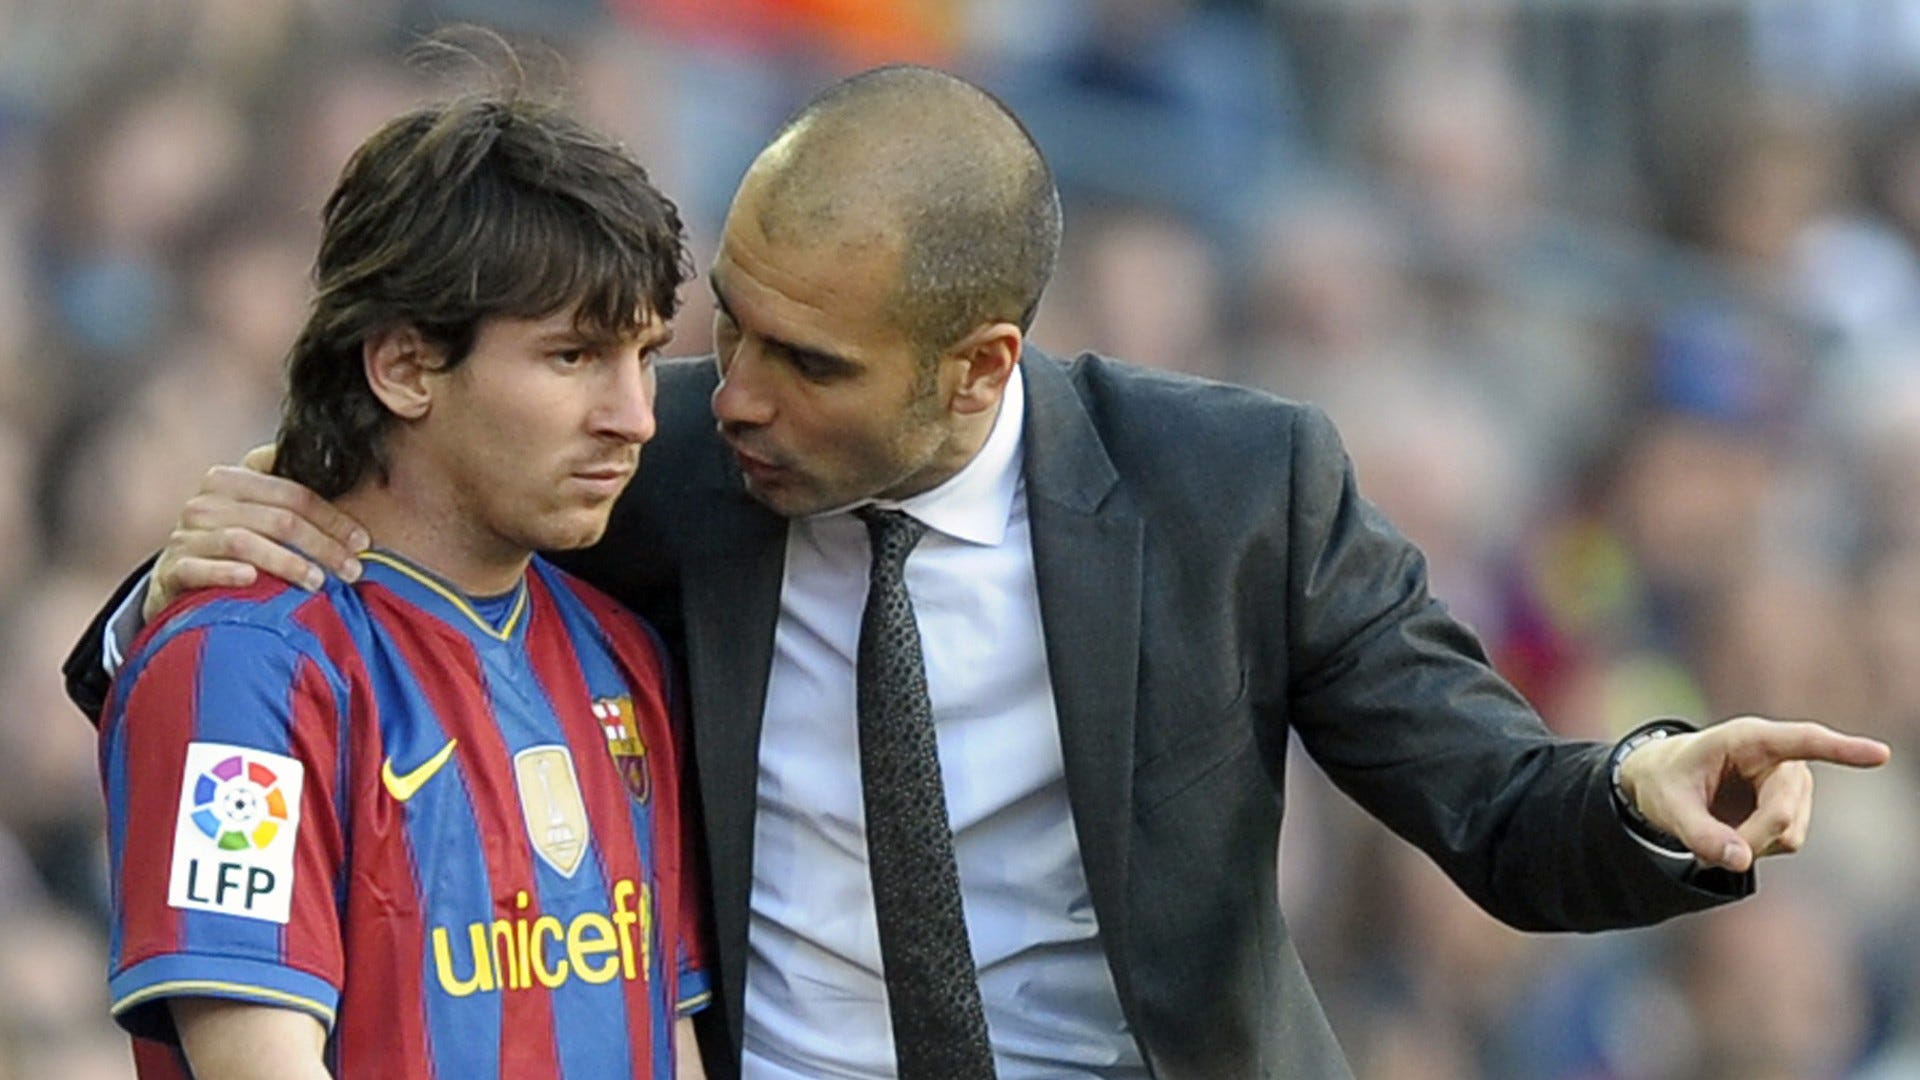
\includegraphics[width=0.7\textwidth]{graphics/messi_pep.jpg}
    \caption{Messi and Guardiola}
    \label{fig:messi_pep}
    \begin{quote}
        \textit{Notes:} 
        The figure shows a picture of Messi and Guardiola.
        \textit{Source:} Eurosport.
    \end{quote} 
\end{figure}


The false nine role was a strategic masterstroke that maximized Messi's
playmaking abilities and goal-scoring prowess.
This tactic went to change the landscape of modern football, with many teams
adopting similar approaches to utilize their creative forwards effectively.


%% CHAPTER TWO %%%%%%%%%%%%%%%%%%%%%%%%%%%%%%%%%%%%%%%%%%%%%%%%%%%%%%%%%%%%%%%%%
\clearpage

\chapter{Messi's International Journey}

%% Update section numbering

\renewcommand{\thesection}{\arabic{chapter}.\arabic{section}} % Use letters for section numbering (undo previous appendix)

\setcounter{table}{0}% Reset table counter
\setcounter{figure}{0}% Reset figure counter

\renewcommand{\thetable}{\arabic{chapter}.\arabic{table}}%
\captionsetup{labelformat=simple}
\renewcommand{\thefigure}{\arabic{chapter}.\arabic{figure}}%
\captionsetup{labelformat=simple}


\section{Introduction}\label{sec:chap2_introduction}

Lionel Messi's international career with the Argentine national team has been
a rollercoaster of emotions, filled with triumphs and heartbreaks.


%% APPENDIX

\section*{\Large\centering{APPENDIX}}

%% Change section numbering for appendix

\setcounter{section}{0}% Reset appendix section counter
\renewcommand{\thesection}{\arabic{chapter}.\Alph{section}}% Use letters for appendix section numbering

\setcounter{table}{0}% Reset table counter
\setcounter{figure}{0}% Reset figure counter

\renewcommand{\thetable}{\arabic{chapter}.\Alph{table}}%
\captionsetup{labelformat=simple}

\renewcommand{\thefigure}{\arabic{chapter}.\Alph{figure}}%
\captionsetup{labelformat=simple}


\section{Messi's International Goals and Statistics}

This appendix provides a detailed breakdown of Lionel Messi's goals and 
statistics for the Argentina national team. 

\begin{table}[h!]
    \centering
    \caption{Lionel Messi's Goals for Argentina National Team}
    \label{tab:messi_argentina_goals}
    \begin{tabular}{cccc}
    \hline
    \textbf{Competition} & \textbf{Goals} & \textbf{Matches} & \textbf{Ratio} \\ \hline
    FIFA World Cup & 13 & 26 & 0.50 \\
    Copa América & 13 & 34 & 0.38 \\
    World Cup Qualifiers & 31 & 65 & 0.48 \\
    International Friendlies & 49 & 54 & 0.90 \\ \hline
    \textbf{Total} & \textbf{106} & \textbf{145} & \textbf{0.73} \\ \hline
    \end{tabular}
\end{table}


\section{Messi's 2022 World Cup Performance}

The 2022 FIFA World Cup witnessed Lionel Messi at his peak, both as a leader 
and as a player.
Appendix Table \ref{tab:messi_worldcup_stats} provides a glimpse into his 
remarkable contributions throughout the tournament. 

His presence on the field was near-constant, matching the tournament's high for 
minutes played. 
While narrowly missing the top scorer title, his seven goals were crucial in 
propelling Argentina to victory. 
He further showcased his playmaking abilities with three assists and a 
significant number of key passes, creating numerous scoring opportunities 
for his teammates.

\begin{table}[h!]
    \centering
    \caption{Messi's 2022 World Cup Statistics}
    \begin{tabular}{lcc}
    \hline
    \textbf{Statistic} & \textbf{Messi's} & \textbf{Tournament High} \\
    & \textbf{Value} & \textbf{(Player)} \\ \hline
    Minutes Played & 690 & 690 (Mbappe) \\
    Goals & 7 & 8 (Mbappe) \\
    Assists & 3 & 3 \\
    Passes Completed & 347 & 684 (Rodri) \\
    Key Passes & 21 & 22 (Griezmann) \\
    Shots & 32 & 32 \\
    Shots From Outside Box & 11 & 11 \\
    Total Dribbles & 34 & 52 (Mbappe) \\
    Successful Dribbles & 15 & 25 (Mbappe) \\
    Tackles & 5 & 26 (Hakimi) \\
    Fouls Won & 22 & 22 \\ \hline
    \end{tabular}
    \label{tab:messi_worldcup_stats}
\end{table}


Beyond the goals and assists, Messi's influence is evident in his overall 
involvement in the game. 
His dribbling skills, despite not topping the charts, remained a constant 
threat to opponents, while his passing accuracy and vision orchestrated 
Argentina's attacking plays. 

These statistics not only reflect Messi's individual brilliance but also 
highlight his role as an inspiration for his team. 
His dedication, leadership, and unwavering pursuit of victory motivated those 
around him, contributing significantly to Argentina's World Cup triumph.
His performance in the 2022 World Cup cemented his place among the greatest 
footballers of all time, leaving an indelible mark on the history of the sport.

%% CHAPTER THREE %%%%%%%%%%%%%%%%%%%%%%%%%%%%%%%%%%%%%%%%%%%%%%%%%%%%%%%%%%%%%%%
% \clearpage

% \chapter{Another chapter title}

% \renewcommand{\thesection}{\arabic{chapter}.\arabic{section}} % Use letters for section numbering (undo previous appendix)

% \setcounter{table}{0}% Reset table counter
% \setcounter{figure}{0}% Reset figure counter

% \renewcommand{\thetable}{\arabic{chapter}.\arabic{table}}%
% \captionsetup{labelformat=simple}
% \renewcommand{\thefigure}{\arabic{chapter}.\arabic{figure}}%
% \captionsetup{labelformat=simple}

% 
\section{Introduction}\label{sec:chap1_intro}
 
Lionel Messi's ascension from a gifted youth prospect to a global football icon 
unfolded over a remarkable period at FC Barcelona.
His time with the Catalan giants serves as a testament to both extraordinary 
talent and unwavering dedication, ultimately elevating him to a status few 
athletes ever achieve. 

This chapter examines the formative years of Messi's legendary career.
By analyzing his performances, his unparalleled success in winning titles, and 
the transformative impact he had on FC Barcelona, the groundwork for 
understanding his enduring influence on the sport is established.
His successes are reflected in titles, such as \textcite{messi2011ucl} 
and \textcite{messi2015ucl}, and in astounding individual performances
\parencite[e.g,][]{messi2009clasico}.

This exploration sets the stage for the dissertation's subsequent analysis of 
Messi's continued evolution throughout his career, 
including the challenges and triumphs he faced beyond Barcelona's hallowed grounds. 

This chapter is organized as follows. 
Section \ref{sec:chap1_background} provides background information on Messi's 
early years at FC Barcelona.
Section \ref{sec:chap1_titles} presents an overview of the titles Messi won 
during his time at the club.
Section \ref{sec:chap1_performance} analyzes Messi's performance metrics during 
his tenure at FC Barcelona.

\section{Background}\label{sec:chap1_background}

Lionel Messi joined FC Barcelona's youth academy, La Masia, at the age of 13.
His prodigious talent was evident from an early age, and he quickly rose through
the ranks of the club's youth system.

Messi made his first-team debut for Barcelona in 2004, at the age of 17, under 
the coaching of Frank Rijkaard.
He quickly established himself as a key player for the club, showcasing his
remarkable dribbling ability, vision, and goal-scoring prowess.

In fact, Messi's first goal for Barcelona came on May 1, 2005, in a match 
against Albacete.
In the 88th minute of the game, Messi received a pass from Ronaldinho and 
skillfully put the ball above the goalkeeper to celebrate his first goal.
At just 17 years and 10 months old, Messi became the youngest goal scorer in 
the history of the club.

\section{Titles}\label{sec:chap1_titles}

During his time at FC Barcelona, Lionel Messi won numerous titles, as depicted
in Table \ref{tab:messi_barca_titles}.
These include multiple La Liga titles, UEFA Champions League titles, and Copa del Rey
titles.

\begin{table}[ht!]
    \centering
    \caption{Lionel Messi's Titles with FC Barcelona}
    \begin{tabular}{|c|c|}
    \hline
    \textbf{Competition} & \textbf{Number of Titles} \\ \hline
    La Liga & 10 \\ \hline
    Copa del Rey & 7 \\ \hline
    UEFA Champions League & 4  \\ \hline
    \end{tabular}
    \label{tab:messi_barca_titles} 
\end{table}
    

His position in the field and playing style evolved over the years, as 
different coaches utilized his talents in various ways.
For example, under Pep Guardiola, Messi played as a false nine, dropping deep
to create space for his teammates and exploit opposition defenses.
This constant evolution and adaptation to different roles on the field
demonstrate Messi's versatility and footballing intelligence, and were 
key to his success at Barcelona.

\begin{table}[ht!]
    \centering
    \caption{Goals and Assists by Lionel Messi Each Year in FC Barcelona}
    \begin{tabular}{ccc}
      \hline
      Season & Goals & Assists \\ \hline
      2004-05 & 9 & 1 \\
      2005-06 & 25 & 8 \\
      2006-07 & 36 & 17 \\
      2007-08 & 40 & 16 \\
      2008-09 & 51 & 38 \\
      2009-10 & 53 & 47 \\
      2010-11 & 55 & 53 \\
      2011-12 & 60 & 73 \\
      2012-13 & 50 & 60 \\
      2013-14 & 46 & 41 \\
      2014-15 & 58 & 57 \\
      2015-16 & 49 & 41 \\
      2016-17 & 52 & 54 \\
      2017-18 & 54 & 45 \\
      2018-19 & 50 & 51 \\
      2019-20 & 44 & 31 \\
      2020-21 & 47 & 38 \\
    \hline
    \end{tabular}
    \label{tab:messi_barca_goals_assists}
\end{table}
  

\section{Performance}\label{sec:chap1_performance}

The performance of Lionel Messi during his tenure at FC Barcelona is 
nothing short of extraordinary.
His goal-scoring and playmaking abilities have earned him numerous 
accolades and titles.
Table \ref{tab:messi_barca_goals_assists} showcases Messi's remarkable 
goal and assist statistics, highlighting his immense contribution to the 
team's success.

Messi had a record-breaking calendar year in 2012, scoring 91 goals in all 
competitions.
This peak performance is illustrated in Figure \ref{fig:messi_goals_xg_2012}, 
which shows the ratio of goals to expected goals (xG) for Messi and other players
in the 2012/13 season.
Messi consistently outperformed his xG, demonstrating his exceptional finishing
ability and efficiency in front of goal.

\begin{figure}[ht!]
    \centering
    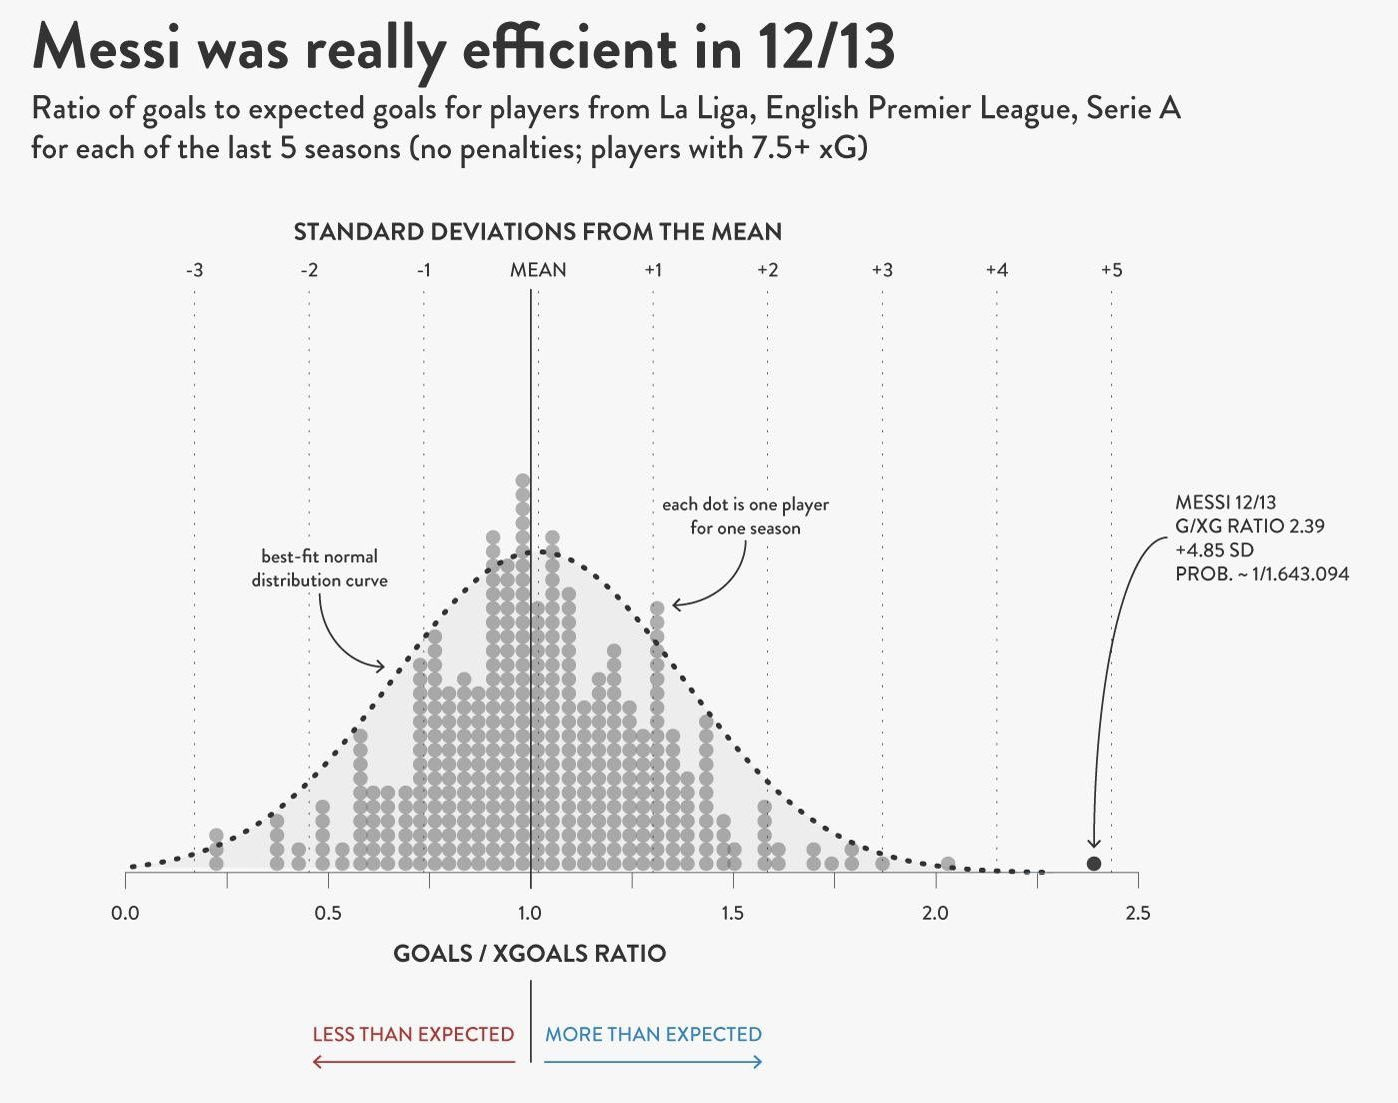
\includegraphics[width=0.7\textwidth]{graphics/messi_2012.jpg}
    \caption{Messi's Exceptional Finishing in 2012/13}
    \label{fig:messi_goals_xg_2012}
    \begin{quote}
        \textit{Notes:} 
        The figure shows the ratio of goals to expected goals (xG) for several 
        players in the 2012/13 season.
        \textit{Source:} Twitter, @xGPhilosophy.
    \end{quote} 
\end{figure}


Messi was coached by some of the best managers in the world during his time at
Barcelona, including Pep Guardiola, Luis Enrique, and Ronald Koeman.
A key aspect of Messi's success was his ability to adapt to different
tactical systems and playing styles.
For instance, Guardiola implemented a ``false nine'' role for Messi, allowing
him to drop deep and create overloads in midfield.
This tatical innovation is explored in Appendix \ref{sec:false_nine}.

Messi's performances resulted in multiple awards and accolades.
Appendix \ref{sec:ballon_dor} provides a summary of Messi's Ballon 
d'Or awards, highlighting his dominance in world football during his time 
at Barcelona.

\subsection{Computing expected goals}

Expected goals (xG) is a statistical metric that quantifies the quality of a
goal-scoring opportunity.
It is calculated based on various factors such as shot location, shot angle,
and type of shot.

The formula for calculating xG is as follows:
\begin{equation}
    xG = \sum_{i=1}^{n} P(G_i) \times G_i
\end{equation}
where $P(G_i)$ is the probability of scoring from a given shot $i$, and 
$G_i$ is the number of goals scored from that shot.
The shot location, shot angle, and type of shot are used to determine the
probability of scoring from a given shot.

By comparing a player's actual goals to their expected goals, analysts can
assess the player's finishing ability and efficiency in front of goal.
This metric provides valuable insights into a player's performance and can
help coaches and analysts make data-driven decisions.

\section{Messi's Departure from Barcelona}\label{sec:messi_departure}

Despite the deep connection between Messi and FC Barcelona, a complex 
set of circumstances led to his unexpected departure from the club in 2021.
Financial constraints within Barcelona, coupled with LaLiga's salary cap 
restrictions, made it impossible to renew Messi's contract.
Even with substantial salary concessions on Messi's part, the club could 
not comply with the league's financial regulations. 

This unforeseen turn of events marked a shocking end to an era that had 
defined both the player and the club.
Messi's exit underscored the complexities of modern football, 
highlighting the interplay between sporting ambition and financial 
considerations.


% %% APPENDIX

% \section*{\Large\centering{APPENDIX}}

% %% Change section numbering for appendix

% \setcounter{section}{0}% Reset appendix section counter
% \renewcommand{\thesection}{\arabic{chapter}.\Alph{section}}% Use letters for appendix section numbering

% \setcounter{table}{0}% Reset table counter
% \setcounter{figure}{0}% Reset figure counter

% \renewcommand{\thetable}{\arabic{chapter}.\Alph{table}}%
% \captionsetup{labelformat=simple}

% \renewcommand{\thefigure}{\arabic{chapter}.\Alph{figure}}%
% \captionsetup{labelformat=simple}

% 
\section{Messi's International Goals and Statistics}

This appendix provides a detailed breakdown of Lionel Messi's goals and 
statistics for the Argentina national team. 

\begin{table}[h!]
    \centering
    \caption{Lionel Messi's Goals for Argentina National Team}
    \label{tab:messi_argentina_goals}
    \begin{tabular}{cccc}
    \hline
    \textbf{Competition} & \textbf{Goals} & \textbf{Matches} & \textbf{Ratio} \\ \hline
    FIFA World Cup & 13 & 26 & 0.50 \\
    Copa América & 13 & 34 & 0.38 \\
    World Cup Qualifiers & 31 & 65 & 0.48 \\
    International Friendlies & 49 & 54 & 0.90 \\ \hline
    \textbf{Total} & \textbf{106} & \textbf{145} & \textbf{0.73} \\ \hline
    \end{tabular}
\end{table}


\section{Messi's 2022 World Cup Performance}

The 2022 FIFA World Cup witnessed Lionel Messi at his peak, both as a leader 
and as a player.
Appendix Table \ref{tab:messi_worldcup_stats} provides a glimpse into his 
remarkable contributions throughout the tournament. 

His presence on the field was near-constant, matching the tournament's high for 
minutes played. 
While narrowly missing the top scorer title, his seven goals were crucial in 
propelling Argentina to victory. 
He further showcased his playmaking abilities with three assists and a 
significant number of key passes, creating numerous scoring opportunities 
for his teammates.

\begin{table}[h!]
    \centering
    \caption{Messi's 2022 World Cup Statistics}
    \begin{tabular}{lcc}
    \hline
    \textbf{Statistic} & \textbf{Messi's} & \textbf{Tournament High} \\
    & \textbf{Value} & \textbf{(Player)} \\ \hline
    Minutes Played & 690 & 690 (Mbappe) \\
    Goals & 7 & 8 (Mbappe) \\
    Assists & 3 & 3 \\
    Passes Completed & 347 & 684 (Rodri) \\
    Key Passes & 21 & 22 (Griezmann) \\
    Shots & 32 & 32 \\
    Shots From Outside Box & 11 & 11 \\
    Total Dribbles & 34 & 52 (Mbappe) \\
    Successful Dribbles & 15 & 25 (Mbappe) \\
    Tackles & 5 & 26 (Hakimi) \\
    Fouls Won & 22 & 22 \\ \hline
    \end{tabular}
    \label{tab:messi_worldcup_stats}
\end{table}


Beyond the goals and assists, Messi's influence is evident in his overall 
involvement in the game. 
His dribbling skills, despite not topping the charts, remained a constant 
threat to opponents, while his passing accuracy and vision orchestrated 
Argentina's attacking plays. 

These statistics not only reflect Messi's individual brilliance but also 
highlight his role as an inspiration for his team. 
His dedication, leadership, and unwavering pursuit of victory motivated those 
around him, contributing significantly to Argentina's World Cup triumph.
His performance in the 2022 World Cup cemented his place among the greatest 
footballers of all time, leaving an indelible mark on the history of the sport.

%% BIBLIOGRAPHY %%%%%%%%%%%%%%%%%%%%%%%%%%%%%%%%%%%%%%%%%%%%%%%%%%%%%%%%%%%%%%%%

\printbibliography[title={BIBLIOGRAPHY}]

\end{document}
